非常に多くの分野で活用されるようになったDeepLearning技術だが,モデルの性能向上に伴い計算に必要な資源も増加している.

\begin{table}[H]
	\caption{FLOPs vs Weights}
	\label{table:flops_vs_weights}
	\centering
	\begin{tabular}{lll}
		\hline
		Model Name & FLOPs & Weights \\ 
		\hline \hline 
		Xception & 8357403496 & 22801424 \\ 
		VGG16 & 15470264320 & 138357544 \\ 
		VGG19 & 19632062464 & 143667240 \\ 
		ResNet50 & 3857973248 & 25530472 \\ 
		ResNet101 & 7570194432 & 44496488 \\ 
		ResNet152 & 11282415616 & 60117096 \\ 
		InceptionV3 & 5713216096 & 23800136 \\ 
		InceptionResNetV2 & 13155794016 & 55782920 \\ 
		MobileNet & 568740352 & 4210088 \\ 
		MobileNetV2 & 300774272 & 3470760 \\ 
		DenseNet121 & 2834161664 & 7895208 \\ 
		DenseNet169 & 3359843328 & 13991080 \\ 
		DenseNet201 & 4291365888 & 19784872 \\ 
		NASNetMobile & 563638816 & 5253240 \\ 
		NASNetLarge & 23783414658 & 88556482 \\ 
		EfficientNetB0 & 388121280 & 5246532 \\ 
		EfficientNetB1 & 690912160 & 7732136 \\ 
		EfficientNetB2 & 998832224 & 9042426 \\ 
		EfficientNetB3 & 1836129536 & 12145936 \\ 
		EfficientNetB4 & 4413319168 & 19216416 \\ 
		EfficientNetB5 & 10306979360 & 30217048 \\ 
		EfficientNetB6 & 19136716704 & 42816272 \\ 
		EfficientNetB7 & 37868782912 & 66037240 \\ 
		EfficientNetV2B0 & 719342144 & 7079096 \\ 
		EfficientNetV2B1 & 1198640192 & 8069980 \\ 
		EfficientNetV2B2 & 1700157088 & 10013798 \\ 
		EfficientNetV2B3 & 3015809440 & 14249190 \\ 
		EfficientNetV2S & 8375340032 & 21304616 \\ 
		EfficientNetV2M & 24609813184 & 53847324 \\ 
		EfficientNetV2L & 56127521408 & 118002696 \\ 
		ConvNeXtTiny & 25491808974 & 27011848 \\ 
		ConvNeXtSmall & 50982829662 & 48625672 \\ 
		ConvNeXtBase & 90635773534 & 85772648 \\ 
		ConvNeXtLarge & 203929679454 & 191474728 \\ 
		ConvNeXtXLarge & 362540942942 & 339054312 \\ 
		\hline
	\end{tabular}
\end{table}

\begin{figure} [H]
	\begin{center}
		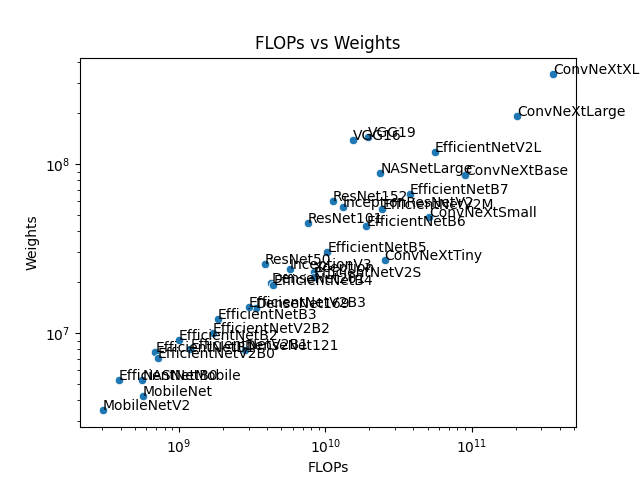
\includegraphics[clip, height=12cm, bb=-60 0 640 480]{data/figure/models_info.png}
		\caption{モデルごとのFLOPsとWeights}
		\label{flops_vs_weights}
	\end{center}
\end{figure}


計算機の資源,特にGPUやスーパーコンピュータの性能も向上しているが,スマートフォンやスマートカメラなど計算資源が限られているエッジデバイスでは,実行可能なモデルも制限される.

% --- T.B.D ---
%市場規模
% 世界市場
%  ✓エッジ型人工知能チップの市場規模は2030年に132億米ドルに達すると予測~最新予測 https://newscast.jp/news/4431496
%  ✓エッジコンピューティング市場規模、2030年に1559億ドル http://www.ex-press.jp/lfwj/lfwj-news/lfwj-biz-market/52519/
%  ✓AIエッジコンピューティング市場、2030年に596億ドル http://ex-press.jp/lfwj/lfwj-news/lfwj-biz-market/45075/
%  ✓エッジ AI プロセッサ市場(Edge AI Processor Market)に関する調査は、2023年の市場のランドスケープを理解するために実施されました。 https://prtimes.jp/main/html/rd/p/000002320.000072515.html
%  ✓エッジ AI ハードウェア市場 - 成長、トレンド、COVID-19 の影響、および予測 (2023 - 2028) https://www.mordorintelligence.com/ja/industry-reports/edge-ai-hardware-market
%  ✓エッジAIソフトウェアの市場規模、2026年に18億3500万米ドル到達予測 https://www.value-press.com/pressrelease/267210
%  ✓エッジAIソフトウェア市場、2027年まで20.3%の成長率を予想 https://aismiley.co.jp/ai_news/edge-ai-software-market-expects-20-3-growth-by-2027/
%  ✓政府機関におけるエッジAIの市場規模、2032年までに30億米ドル到達予測 https://www.mapion.co.jp/news/release/dn0000270836-all/
%  ✓エッジAIコンピューティング市場を予想、2025年度には413億円に拡大 https://news.mynavi.jp/techplus/article/20211214-2227346/
% 国内市場
%  ✓【エッジAIの活用事例】AIカメラからFA機器まで市場規模は拡大の一途 https://standard-dx.com/post_blog/edge-ai
%  ✓本格的な導入が進む国内のAI(人工知能)ビジネス市場を調査 https://www.fuji-keizai.co.jp/press/detail.html?cid=19039
%  ×ミック経済研究所、マーケティング資料「エッジAIコンピューティング市場の実態と将来展望 2021年度版」を発刊 https://www.nikkei.com/article/DGXLRSP623718_U1A211C2000000/
%  ✓国内エッジAI市場は前年比70.8%増、今後の成長ドライバーはAIエンジン─デロイト トーマツ ミック研 https://it.impress.co.jp/articles/-/24005
%  ✓エッジ AI プロセッサ市場(Edge AI Processor Market)に関する調査は、2023年の市場のランドスケープを理解するために実施されました。 https://prtimes.jp/main/html/rd/p/000002320.000072515.html
%  ×データセンター市場及び クラウドサービス市場の動向 https://www.soumu.go.jp/johotsusintokei/whitepaper/ja/r05/pdf/n4800000.pdf
%  ✓AIの拡大と活用動向 https://www.toshiba-dme.co.jp/dme/dig/edge_solution/trend.htm
%  ✓IDC Japan、2023年以降の国内AIシステム市場予測を発表 https://aismiley.co.jp/ai_news/idc-japan-2023/
%  ×富士キメラ総研 AIビジネス国内市場調査 2025年には2兆円規模に拡大 DXに不可欠な要素技術として利用増加 https://www.automation-news.jp/2021/07/57280/
% 技術トレンド
%  ✓2023 年に注目すべきエッジ AI の 5 つのトレンド https://blogs.nvidia.co.jp/2023/01/17/edge-ai-trends-2023/
%  エッジAIカメラの活用から市場動向まで:スマートセキュリティと画像認識技術の最新トレンドを徹底解説 https://www.morphoai.com/post/edge-ai-content
%  エッジAI分野における優位性の獲得 https://www.jp.kearney.com/issue-papers-perspectives/gaining-the-edge-in-edge-ai
%  エッジAI発展に重要な「インメモリコンピューティング」 https://eetimes.itmedia.co.jp/ee/articles/2109/30/news084.html
%  エッジAIとは?5つの活用シーンと10社の開発事例を紹介 https://ainow.ai/2020/02/21/183186/
%  A.T.カーニー、エッジAI市場における勝利の方程式を導く論考「エッジAI分野における優位性の獲得」を公開 https://ledge.ai/articles/kearney-edge-ai
%業界団体
%	TinyML
%
%企業
%  エッジAIカメラの活用から市場動向まで:スマートセキュリティと画像認識技術の最新トレンドを徹底解説 https://www.morphoai.com/post/edge-ai-content
%  TI Edge AI Cloud https://dev.ti.com/edgeai/?utm_source=google&utm_medium=cpc&utm_campaign=epd-null-null-58700008186542725_EdgeAI_Dev_rsa-cpc-pp-google-jp_int&utm_content=EdgeAI_Dev&ds_k=%E3%82%A8%E3%83%83%E3%82%B8+AI&DCM=yes&gclid=Cj0KCQjwuNemBhCBARIsADp74QRb9Mx3n5koyT99HvoPdK97xdrHLeFVCg1WCJ1nEaJagx5JH9giDhsaAlsjEALw_wcB&gclsrc=aw.ds
%  エッジAIコンサルティングサービス https://www.araya.org/service/edgeaiconsulting/?utm_source=google&utm_campaign=edgeai&utm_medium=cpc&gclid=Cj0KCQjwuNemBhCBARIsADp74QR13i96ZIk77RCoSMZfKjfE2cxfO-JxD4RIJ34oPDFb7fzgh9GbIpcaApKhEALw_wcB
%  国内シェアNo.1エッジAIプラットフォーム https://www.idein.jp/ja
%  AI開発に強い開発会社、プロ厳選の21社!【2023年最新版】 https://ai-market.jp/services/ai_development_company/




